\documentclass[12pt]{article}
\usepackage{geometry}
\usepackage{cancel}
\usepackage{graphicx}
\usepackage{sectsty}
\pagenumbering{gobble}
%sectionfont{\centering}
\geometry{
	letterpaper,
	left= 1in,
	right=1in,
	top=20mm,
}
\usepackage{amssymb,amsmath}
\begin{document}
	\nopagebreak
\section*{Model}
	\[\hat{y}=11.9524+0.0029\cdot \hat{x},\quad \text{where}\quad  \hat{y}=\ln (\text{price})\text{ and } \hat{x} = \text{sqft\_living}^{0.78}  \]
\section*{Explanation of the Model}
The model has the sample intercept of \(11.9524\) and the slope of \(0.0029\).  To interpret the slope, we have to transform \(\hat{x}\) and \(\hat{y}\) towards original {\it sqft\_living} and {\it price}. Let \(x\) = {\it sqft\_living}  and \(y\) = {\it price} for the derivation. We have  \(\hat{x} = x^{0.78}\) and \(\hat{y} = \ln (y)\implies y  = e^{\hat{y}}\). Suppose the original sqft\_living is \(x_1\) and it moved up to \(x_2\), then we have the following :
\begin{align*}
	y_1 =& e^{\hat{y}_1 }= e^{11.9524+0.0029\cdot x_1^{0.78}}  = e^{11.9524}\cdot e^{0.0029\cdot x_1^{0.78}}\\
	y_2 =& e^{\hat{y}_2 }= e^{11.9524+0.0029\cdot x_2^{0.78}}  = e^{11.9524}\cdot e^{0.0029\cdot x_2^{0.78}}
\end{align*}
To understand the change in {\it price} in percents we will use the following formula:

\begin{align*}
100 \times \left[\frac{y_2-y_1}{y_1} \right] =& 100 \times \left[\frac{y_2}{y_1} - 1\right] = 100\times \left[\frac{ \cancel{e^{11.9524}}\cdot e^{0.0029\cdot x_2^{0.78}}}{\cancel{e^{11.9524}}\cdot e^{0.0029\cdot x_1^{0.78}}} -1 \right] \\
=& 100 \times \left[ e^{0.0029\left( x_2^{0.78} - x_1^{0.78} \right)} -1 \right]
\end{align*}
For example, if the {\it sqft\_living} is \(1000ft\) and we increase it to \(1100\), we will get change in price of \(100\times \left[e^{0.0029(1100^{0.78}-1000^{0.78})}-1\right] \approx 5.02\% \). In this particular example \(10\%\) change in sqft\_living starting from \(x_1 = 1000ft\) forces \(5.02\%\) change in price.
\section*{Check Statistical Hypotheses of the Regression}
\subsection*{Linearity:}
\textbf{The Null Hypothesis:  The model is linearly predicted by the feature,\\
The Alternative Hypothesis:  The model is not linearly predicted by the feature.}\\
Our p-value for this model is \(p=0.877 > 0.05 = \alpha\). Thus, we don't have enough evidence to reject \textbf{The Null Hypothesis} and  we conclude that our model satisfies Linearity Assumption.
\newpage
\subsection*{Normality Assumption for Errors}
To check Normality, I used the following checks:
\begin{enumerate}
	\item QQ-Plot\\
	\begin{center}
		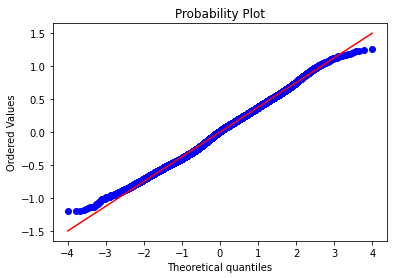
\includegraphics[width=2in]{qq_plot_linear_model}
	\end{center}
\end{enumerate}
\end{document}
